% -*- encoding: UTF8 -*-
%
%%*****************************************************************************
%---------------------------------------Measurement Results --------------------------------------
%%*****************************************************************************
%
\chapter{Experimental Evaluation}
\label{Ch:Measurements}	

The following pages describe the performance of the OCT scanner demonstrator probe. First, the optomechanical characteristics of three manufactured probes are compared with their expected values. Later, a set of driving parameters optimized for each probe is used to image a sample using spiral scanning. The challenges and solutions associated with this method are discussed, highlighting the different data processing methods. Eventually, OCT measurements of biological samples are presented.

%%*****************************************************************************
\section{Fiber scanner characterization}
%%*****************************************************************************

Three single modality demonstrator probes were assembled to test the repeatibility of the process.  For each probe, a characterization step was performed in order to measure its resonance frequency, laser coupling efficiency, backreflectivity and maximum unobstructed field of view. These results are summarized in \autoref{tab:char}.

\begin{table}[h!]\centering
\caption{Optomechanical characteristics of three assembled single modality probes compared with their expected values, calculated for a cantilever length of \SI{4.5}{\milli\meter}.}
\begin{tabular}{rcccc}
& 							\textbf{Design Value}&\textbf{Probe 1} & \textbf{Probe 2} & \textbf{Probe 3} \\ 
\hline
Cantilever Length [\SI{}{\milli\meter}] & 	4.5		& 	4.45 	& 	4.44	& 	4.10	\\
Field of View [\SI{}{\milli\meter}]		&	1.3		&	1.1	 	&	1.2 	& 	1.2  	\\ 
Resonant Frequency [\SI{}{\hertz}]  	&	762		& 	744		&	765 	& 	842 	\\ 
Coupling Efficiency  					&	-		& 	0.53	&	0.61 	&	0.58 	\\ 
Backreflectivity [\%] 					&	-		& 	0.011	&	0.004 	& 	0.018 	\\ 
\hline
\end{tabular} 
\label{tab:char}
\end{table}
\begin{itemize}


\item \textbf{Cantilever Length:} The cantilever length was varied between \SI{4.10}{\milli\meter} and \SI{4.45}{\milli\meter} to test the behavior of the scanner under different parameters. 

\item \textbf{Field of View:} At a certain scanning amplitude, the laser beam becomes shadowed by the edges of the optical components. In the case of the single modality probe, this happens due to the walls of the housing, which by design limit the FOV to \SI{1.3}{\milli\meter}. Any misalignment between the optical axis of the scanner and the symmetry axis of the housing further reduces the FOV due to decentering.

\item \textbf{Resonant Frequency:} The resonance frequency was measured by driving the scanner with a sweeping sinusoidal signal and observing the amplitude of oscillation An example of such response can be seen in \autoref{fig:bode}. The variability of the cantilever length explains the change of the resonant frequency: shorter cantilevers exhibit higher resonance frequency, as their stiffness is higher. It can be seen that for Probes 1 and 2, whose cantilever length is close to the designed \SI{4.5}{\milli\meter}, their resonant frequency is within 3\% of the expected \SI{762}{\hertz}. 

\item \textbf{Coupling Efficiency:} This value was calculated by measuring the intensity of the beam exiting the probe divided by the power of the light source at its output fiber connector. Thus, it includes the losses from the FC/APC fiber connector, fiber interfaces and backreflections. It is believed that the main source of loss is the connector, which has variable losses up to 30\%, depending on the quality of the polishing of the fiber facet and any surface imperfection or contamination. 

\item \textbf{Backreflectivity:} In order to measure the backreflected light intensity it is necessary to send and receive light through the scanning fiber. To achieve this, is it possible to reuse an OCT measurement setup with some modifications. As seen in \autoref{fig:confSetup}, broadband infrared light with a center wavelength of $\lambda_o = \SI{1311}{\nano\meter}$ and a bandwidth of $\Delta \lambda = \SI{90}{\nano\meter} $ from an SLED is coupled to a circulator, which forwards it to the probe. Any light which is backreflected inside the probe, together with backscattered light from the sample is coupled back to the fiber and forwarded by the circulator to the photodetector. In case that the probe is pointing to empty space, only light backreflected from the optical components is measured. By dividing this intensity by the source intensity and taking into account the coupling efficiency of the system, the backreflectivity was measured to be well controlled under 0.02\%. The variability within probes can be attributed to differences in alignment and gluing of the fiber and GRIN lens or connector backreflections.

\end{itemize}

\begin{figure}[h!]\centering \includegraphics[width=12cm]{figures/50_Measurements/conf/setup/confSetup.pdf}
      \caption{Setup used to measure the backreflectivity of the probe and for fiber-optical confocal scanning microscopy. Light originating from the SLED is coupled to the probe through the circulator, while the backscattered light from the probe and sample is coupled to the photodetector.}
      \label{fig:confSetup}
\end{figure}

%%*****************************************************************************
\section{Dynamic behavior of the scanner}
%%*****************************************************************************
\label{sec:whirling}
The use of fiber scanners for imaging involves the challenge of whirling, identified already in the first fiber scanner implementations \cite{Seibel2001}.

This effect can be explained as follows: If a cantilever is rotationally symmetric, it will exhibit a single transversal resonant frequency. In this case, according to linear theory, if the base is excited in only one plane, the fiber will also only vibrate in that plane. But if a cantilever shows a small misalignment or non symmetric cross section -- as expected in any real world implementation -- it will exhibit two different frequency responses with peaks $f_x$ and $f_y$, corresponding to two planes of symmetry or eigendirections $x,y$, as can be seen in the example from \autoref{fig:bode}a. Far away from resonance the difference between axes is minimal. But close to resonance, these nonlinear effects create a cross-plane instability in which excitation of the base of the resonator in the $x$ direction can lead to oscillations in both $x$ and $y$ directions. This effect can be seen in the whirl plots of \autoref{fig:bode}b. 

\begin{figure}[h!]\centering 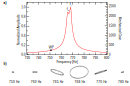
\includegraphics{figures/50_Measurements/bode/bodeWhirl.pdf}
      \caption{\textbf{a)} Dynamic behavior of the scanner in \textit{Probe 2} under harmonic excitation. The two eigenfrequencies corresponding to the main axes of the scanner are marked as $f_\mathrm{x} = \SI{765.8}{\hertz}$ and $f_\mathrm{y} = \SI{768.1}{\hertz}$.
      The Working Point WP shows a gain of 220. 
      The right axis shows the mechanical gain due to resonance, defined as the ratio of the displacement of the GRIN tip to the displacement of the piezoelectric tube tip.
      \textbf{b)} Whirl patterns obtained by exciting the scanner in the $x$ direction with different harmonic frequencies while measuring the position of the fiber tip. }
      \label{fig:bode}
\end{figure}

Therefore, for the imaging experiments, the scanner operates at a working point \textit{WP} far away from the resonance, in order to minimize the effect of whirling, but with a gain high enough to achieve the required amplitude of oscillation.


%%*****************************************************************************
\section{Laser scanning imaging}
%%*****************************************************************************
This section explains how it is possible to use the single modality probe for laser scanning imaging (LSI) and use the acquired images to assess its lateral resolution and depth of field. As OCT uses the concept of LSI to recreate volumetric images, these results are also representative for OCT imaging.

\subsection{Imaging}
The setup used to measure the backreflectivity of the probe, shown in \autoref{fig:confSetup}, can be used directly for LSI. While the probe scans an object with a spiral pattern defined by the driving voltage datapoints $(\mathbf{u_x}[n], \mathbf{u_y}[n])$, the data acquisition system (DAQ) samples a stream of intensities at the photodetector $\mathbf{I}[n]$, as shown in \autoref{fig:confPlotting}a. As these signals are generated and acquired synchronously, we expect that the intensity $\mathbf{I}[i]$ corresponds to a point in object space linearly related to the driving voltage of the piezoelectric scanner: $(x, y) = K_\mathrm{mech}(\mathbf{u_x}[i], \mathbf{u_y}[i])$, where $K_\mathrm{mech}$ is a mechanical constant.

\begin{figure}[h!]\centering \includegraphics{figures/50_Measurements/conf/proc/Plotting.pdf}
      \caption{Different representations of the same acquired datapoints $\mathbf{I}[n]$ of a USAF 1951 resolution test chart. The full acquired spiral consists of 374 rings of 122 datapoints, adding up to 45500 datapoints measured at \SI{91}{\kilo\hertz} during \SI{500}{\milli\second}. The field of view is \SI{1.1}{\milli\meter}.\\
      \textbf{a}: Point cloud assuming ideal movement of the scanner.
      \textbf{b}: Point cloud after correcting the position of each dot using a lookup table.
      \textbf{c}: Raster image after performing a 2D interpolation from the data in d.}
      \label{fig:confPlotting}
\end{figure}

If all the datapoints $\mathbf{I}_{[n]}$ acquired during a full spiral are plotted as a intensity-coded dot located at the position $K_\mathrm{mech}(\mathbf{u_x}[n], \mathbf{u_y}[n])$, the resultant image would look as in \autoref{fig:confPlotting}a: distorted. Notice how the dot plot defines two overlaid whirling images. This proves that the previous assumption of linearity is not valid, and thus the relationship between $(\mathbf{u_x}[i], \mathbf{u_y}[i])$ and $(\mathbf{x}[i], \mathbf{y}[i])$ is neither linear nor simple. This is the result of whirling, as discussed in \autoref{sec:whirling}. There are two general methods to overcome this problem:

The first one involves closed loop operation, where the current position of the scanner is measured inside the probe and used by the plotting system to correct for the distortion \cite{Yeoh2014}. 

The open loop alternative, used in this work, assumes that the distortion pattern is constant for a given driving signal. Then, the distorted spiral pattern $(x[i], y[i])$ can be measured after the assembly of the probe using a position sensitive device (PSD) and stored as a calibration lookup table.
Once this calibration step is performed, any further frame is plotted by assigning a position $(\mathbf{x}[i], \mathbf{y}[i])$ to every measured intensity $\mathbf{I}[n]$, as depicted in \autoref{fig:confPlotting}b, resulting in a distortionless dot plot. This procedure can be performed in real time.

The dot plots which are obtained from spiral scanners have the inconvenient of non-uniform sampling, as can be seen in \autoref{fig:calib}. Thus, to ease the further processing of the acquired images, it is beneficial to convert the non-uniform dot plot into a cartesian raster image. This can be performed by 2D interpolation, resulting in \autoref{fig:confPlotting}c.


\begin{figure}[h!]\centering \includegraphics[width=6cm]{figures/50_Measurements/conf/proc/samplingDensity.png}
      \caption{Sampling points of the scanner during a complete spiral cycle measured using a PSD. Notice the non-uniform sampling. Each one of the 45500 dots represents a sample point in object space. The coordinates of each point $(\mathbf{x}[i], \mathbf{y}[i])$ are used in a LUT to correct for the inherent sampling distortion characteristic of fiber scanners.}
      \label{fig:calib}
\end{figure}


\subsection{Lateral resolution measurement}
The optical performance of the scanner is qualitatively evaluated by capturing a SLI image of a USAF 1951 resolution test chart with a spiral scanning pattern using the setup described in \autoref{fig:confSetup}. As can be seen in \autoref{fig:confPlotting}c, element 4 of group 4 is resolved, indicating a resolution of 22 line pairs/mm or \SI{45}{\micro\meter}. 

A more robust method for the calculation of the optical resolution is detailed in \autoref{ssec:PSFMTF}: by manually scanning the focus of the probe over a sharp chromium edge of the test chart, the edge spread function (ESF) shown in \autoref{fig:MTF}a is obtained. By performing a spatial derivative followed by a Fourier transform of the ESF, the MTF can be obtained, plotted in \autoref{fig:MTF}b. Based on this curve the lateral resolution of the OCT beam path was determined at 21 line pairs/mm or \SI{47.6}{\micro\meter}. This value is very close to the theoretical resolution, calculated in \autoref{sec:ZEMAX} as 23.3 line pairs/mm or \SI{43}{\micro\meter}.
\begin{figure}[h!]\centering 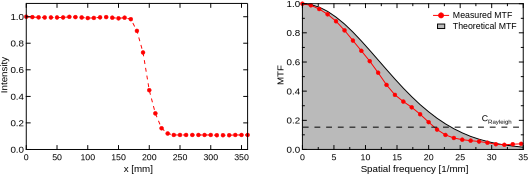
\includegraphics{figures/50_Measurements/conf/res/confResMeas.pdf}
      \caption{Left: Measured edge spread function (ESF) of the OCT beampath for the center of the field of view. 
      Right: Corresponding MTF compared with the theorical limit using the theory from \autoref{ssec:LSI}.}
      \label{fig:MTF}
\end{figure}
A good concordance is observed between the shape of the analytical and the measured MTF curves of the scanning modality. However, the overall performance is reduced by 10\% compared to the simulation. This deviation can be explained by small misalignments of the optical components induced by the process tolerances of the 3D-printed housing and the assembly process. Since a better alignment can be achieved in the silicon micro bench due to the higher precision of the MEMS processes a better match between simulation and reality can be expected for the multimodal probe.

%%*****************************************************************************
\subsection{Depth of field measurement}
%%*****************************************************************************
The depth of field (DOF) of the OCT imaging system can me determined by measuring how much light is backreflected upon a mirror while displacing it though the z axis. The results from this experiment are plotted in \autoref{fig:FWHM}, where a full width half maximum (FWHM) DOF of \SI{3.5}{\milli\meter} is calculated. 

\begin{figure}[h!]\centering \includegraphics{figures/50_Measurements/conf/res/PSFz.pdf}
      \caption{Measurement of the axial resolution of the single modality probe. The intensity of the light coupled back into the optical system after reflection on a mirror is plotted against the manual translation of the mirror by $\pm \SI{4.5}{\milli\meter}$ from the focal plane of the probe. }
      \label{fig:FWHM}
\end{figure}




%%*****************************************************************************
\clearpage
\section{OCT imaging}
%%*****************************************************************************

The OCT characterization was performed using a swept-source OCT system property of the Medical University Vienna. This system, represented in \autoref{fig:OCTsetup} operates with a center wavelength of \unit[1.34]{\textmu m}, a bandwidth of \unit[37]{nm} and a theoretical axial resolution in air of \unit[26.9]{\textmu m}.

\begin{figure}[h!]\centering \includegraphics[width=12cm]{figures/50_Measurements/oct/octSetupVienna.pdf}
      \caption{Medical University Vienna swept-source OCT system. Light originating from a swept-source laser is coupled to a balanced interferometer, where the optical path difference between the sample and the reference arm creates an interferogram which is converted to an electrical signal in a balanced detector.}
      \label{fig:OCTsetup}
\end{figure}

The first OCT tests were performed as a proof of concept. Circular B-Scans of a colon polyp and a fingertip were captured with the single modality demonstrator, shown in \autoref{fig:B-Scan}. 
\begin{figure}[h!]\centering 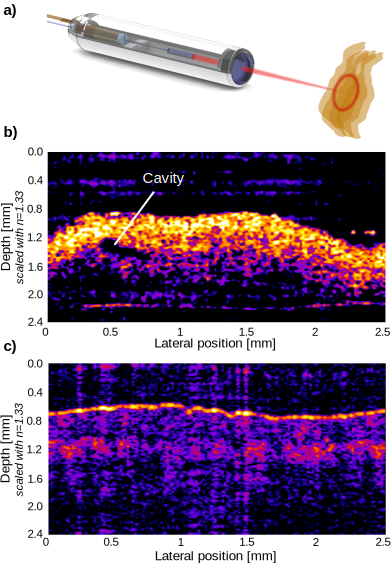
\includegraphics{figures/50_Measurements/oct/OCT_Measurement_arrangement.pdf}
      \caption{a) Illustration of the measurement arrangement for the circular B-Scan used as a proof of concept of OCT. b) Image of a circular OCT B-Scan of a colon polyp with a diameter $d=0.8\,\text{mm}$. Structural changes within the tissue can be detected and at the current state of the investigation the images suggest that blood vessels can be detected.
      c) Image of a circular OCT B-Scan of a human finger tip, where the epidermis, dermis and hypodermis can be tentatively differentiated.}
      \label{fig:B-Scan}
\end{figure}
These preliminary results prove that OCT imaging is possible. But at the same time, the low SNR of these images indicate that the designed system, which has a NA of 0.022, has problems collecting enough backscattered light. Therefore, future implementations of the probe could benefit from a higher NA. In that case, the resolution and collection of light of the system would be increased at the cost of a shorter working distance and a shorter depth of field. 